\chapter{Wprowadzenie}
Rozdział ten został poświęcony przybliżeniu czytelnikowi zasad działania programowania współbieżnego oraz równoległego, a także omówieniu tych mechanizmów w kontekście języków Rust i C++.

Współczesne systemy komputerowe stają się coraz bardziej złożone, a jednocześnie coraz bardziej wydajne dzięki rozwojowi technologii wielordzeniowych i wieloprocesorowych. W tej sytuacji programowanie współbieżne i równoległe zyskało kluczowe znaczenie, umożliwiając pełne wykorzystanie możliwości sprzętowych. Umiejętność projektowania oraz wdrażania aplikacji, które skutecznie zarządzają równoczesnym wykonywaniem wielu zadań, stała się niezbędna dla programistów tworzących oprogramowanie wymagające wysokiej wydajności oraz możliwości dalszego rozwoju \cite{IntroductionToConcurrencyAndParallelism, ConcurrencyInAction, ProgramminInOpenMp, ParallelProgramminginC++withOpenMP}. W niniejszej pracy autor postanowił zbadać podejścia do programowania równoległego jak i współbieżnego zarówno w kontekście języka Rust, jak i C++. Rust jest relatywnie młodym językiem, zaprojektowanym z myślą o bezpieczeństwie pamięci i unikaniu typowych błędów wielowątkowych. Z kolei C++ to język o ugruntowanej pozycji, znany z elastyczności i wysokiej wydajności, co czyni go popularnym wyborem dla aplikacji wymagających precyzyjnego zarządzania zasobami.

Programowanie współbieżne \eng{concurrent programming} oraz programowanie równoległe \eng{parallel programming} to dwa różne, lecz uzupełniające się podejścia, które umożliwiają organizację pracy wielu zadań w aplikacji - poglądowa różnica została zamieszczona na rysunku \ref{fig:concurrent_vs_parallel}. Chociaż często używa się ich zamiennie, ich cechy i cele różnią się znacznie.

\begin{figure}[H]
    \centering
    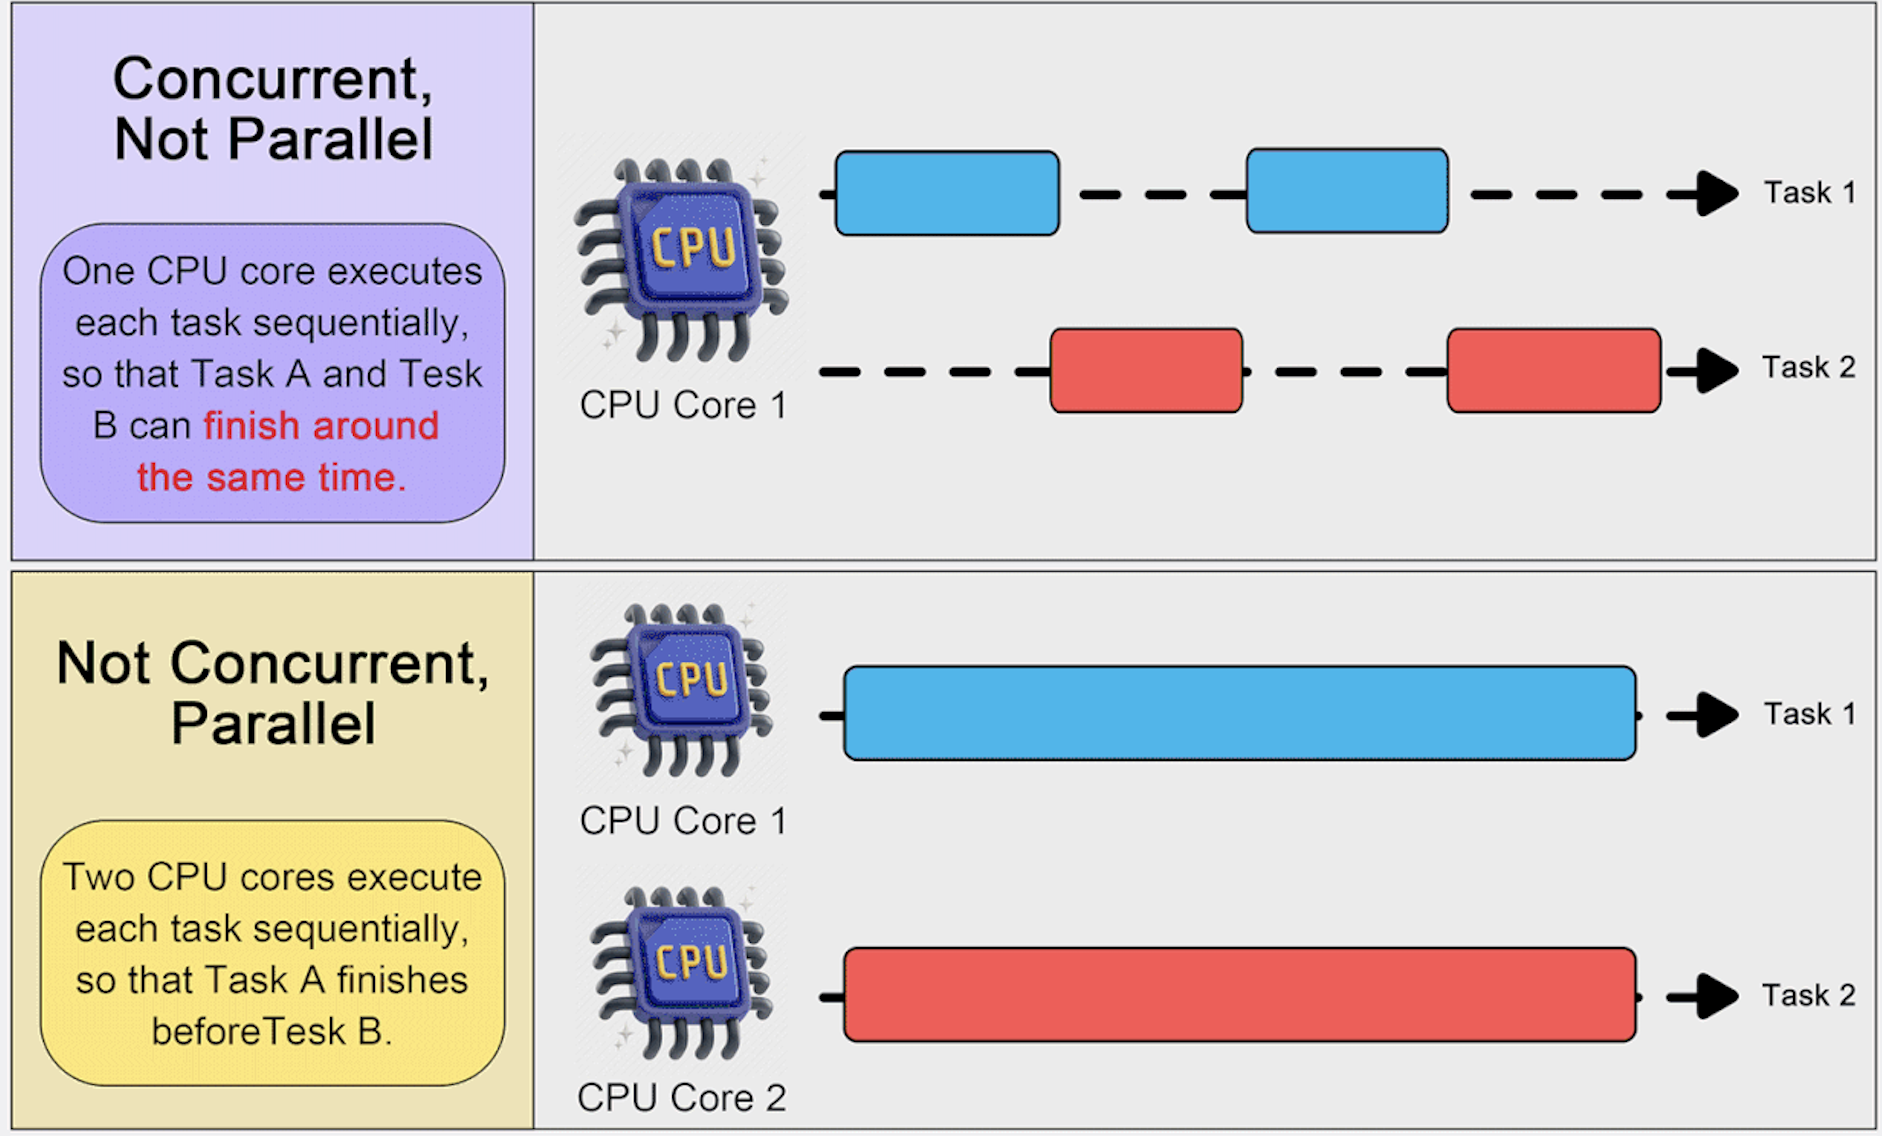
\includegraphics[width=0.8\textwidth]{images/ConcurrentParallelCompare.png}
    \caption{Różnice między wykonywaniem zadań współbieżnie a równolegle \cite{bytebytegoEP108Design}}
    \label{fig:concurrent_vs_parallel}
\end{figure}

\section{Programowanie współbieżne}

Programowanie współbieżne to podejście w projektowaniu aplikacji, które umożliwia równoczesne wykonywanie wielu zadań, choć faktycznie procesor wykonuje tylko jedno zadanie w danej chwili. Dzięki technice tzw. "quasi-równoległości"\ \cite{Paluch} użytkownik ma wrażenie, że zadania te są realizowane jednocześnie, ponieważ procesor przełącza się między nimi w bardzo krótkich odstępach czasu. Takie podejście jest kluczowe w aplikacjach interaktywnych, takich jak gry komputerowe, aplikacje mobilne czy serwisy internetowe, które muszą błyskawicznie reagować na różne zdarzenia (np. żądania użytkowników, kliknięcia czy komunikaty sieciowe) bez zauważalnych opóźnień \cite{MasteringConcurrencyAndParallelProgramming}.

Programowanie współbieżne pozwala na lepsze zarządzanie zadaniami w aplikacjach, które muszą obsługiwać wiele operacji jednocześnie, choć nie zawsze są to zadania wymagające intensywnych obliczeń. Przykładami takich aplikacji mogą być systemy obsługi żądań użytkowników na serwerach, aplikacje multimedialne czy interfejsy graficzne \cite{IntroductionToConcurrencyAndParallelism}.

\subsection{Mechanizmy realizujące współbieżność}
Współbieżność różni się od programowania równoległego tym, że nie wymaga fizycznej wielordzeniowości procesora. Nawet na jednordzeniowym procesorze możliwe jest uzyskanie współbieżności, ponieważ procesor może w bardzo szybki sposób przełączać się między różnymi zadaniami. Tego rodzaju przełączanie nazywane jest "wirtualnym przełączaniem"\ i odbywa się na poziomie systemu operacyjnego, który odpowiedzialny jest za przeprowadzanie tego procesu w sposób niewidoczny dla użytkownika. Dzięki tej technice użytkownik nie zauważa, że procesor w danym momencie wykonuje tylko jedno zadanie, mimo że wiele z nich jest obsługiwanych "po kolei"\ w bardzo krótkich cyklach \cite{ConcurrencyInAction, RustAtomicsAndLocks}.

Kolejnym istotnym mechanizmem, który wspiera współbieżność, jest program szeregujący bądź też planista \eng{scheduler}. Jest odpowiedzialny za zarządzanie dostępem do procesora i przydzielanie zasobów obliczeniowych poszczególnym zadaniom. Dzięki zaawansowanym algorytmom harmonogramowania, system operacyjny decyduje, które zadanie ma być wykonane w danym czasie, jak długo ma trwać jego wykonanie, oraz kiedy procesor ma przełączyć się na inne zadanie. Planista zadań może być dostosowywany w zależności od wymagań aplikacji, co pozwala na osiągnięcie optymalnej wydajności i minimalizację opóźnień \cite{ConcurrencyInAction}.

\subsection{Zastosowania programowania współbieżnego}
Programowanie współbieżne jest niezwykle ważne w aplikacjach, które muszą reagować na różne wydarzenia użytkownika lub zewnętrzne zdarzenia w czasie rzeczywistym. Typowe zastosowania programowania współbieżnego obejmują \cite{ZastosowanieWspolbieznosci, ConcurrencyInAction}:
\begin{itemize}
    \item Aplikacje interaktywne - gry komputerowe, aplikacje mobilne, aplikacje desktopowe, które muszą natychmiast reagować na akcje użytkownika, jak kliknięcia, gesty czy komendy wprowadzane z klawiatury.
    \item Systemy serwerowe - serwisy internetowe, bazy danych, aplikacje chmurowe, które muszą jednocześnie obsługiwać wielu użytkowników, wykonując różne operacje, takie jak przetwarzanie zapytań, zapisywanie danych, czy obsługę sesji użytkowników.
    \item Przetwarzanie zdarzeń w czasie rzeczywistym - systemy monitoringu, systemy alarmowe, aplikacje do analizy danych strumieniowych, które muszą przetwarzać i reagować na dane napływające w czasie rzeczywistym.
    \item Multimedia - odtwarzanie wideo, transmisje strumieniowe, edycja audio i wideo, gdzie aplikacje muszą równocześnie obsługiwać wiele wątków.
\end{itemize}


\subsection{Zalety programowania współbieżnego}
Główne zalety stosowania programowania współbieżnego w aplikacjach to \cite{ProsAndCons, ConcurrencyInAction}:
\begin{itemize}
    \item Zwiększenie responsywności - dzięki szybkiemu przełączaniu między zadaniami aplikacje stają się bardziej responsywne i wydajne, co jest szczególnie ważne w przypadku interfejsów użytkownika oraz aplikacji reagujących na dynamicznie zmieniające się dane.
    \item Lepsze wykorzystanie zasobów procesora - współbieżność pozwala na efektywne wykorzystanie mocy obliczeniowej procesora, nawet w przypadku procesorów jednordzeniowych. Przełączanie między zadaniami pozwala na ich efektywne wykonywanie w krótkich cyklach czasowych.
    \item Skalowalność - aplikacje wykorzystujące współbieżność mogą być łatwiej skalowane na wiele rdzeni procesora lub urządzeń, dzięki czemu mogą obsługiwać większą liczbę użytkowników lub większe ilości danych.
\end{itemize}

\subsection{Wady programowania współbieżnego}
Pomimo wielu korzyści, programowanie współbieżne wiąże się również z pewnymi wyzwaniami \cite{ProsAndCons, HandsOnConcurrencywithRust}:
\begin{itemize}
    \item Złożoność synchronizacji - w przypadku współdzielenia zasobów, takich jak pamięć, konieczne jest odpowiednie zarządzanie dostępem do nich. Błędy synchronizacji mogą prowadzić do problemów takich jak wyścigi danych \eng{race conditions} lub zakleszczenia \eng{deadlocks}, które mogą uniemożliwić poprawne działanie aplikacji.
    \item Problemy związane z wydajnością - chociaż współbieżność pozwala na szybsze przetwarzanie wielu zadań, jej realizacja może prowadzić do narzutów związanych z przełączaniem kontekstu i synchronizacją. W aplikacjach o dużym stopniu współzależności zadań, narzut ten może negatywnie wpływać na wydajność.
    \item Trudności w debugowaniu - aplikacje współbieżne są trudniejsze do debugowania, ponieważ błędy mogą występować sporadycznie i w zależności od kolejności przełączania wątków, co utrudnia ich wykrywanie i naprawę.
\end{itemize}

\section{Programowanie równoległe}

Programowanie równoległe to technika, która umożliwia równoczesne wykonywanie wielu zadań, wykorzystując wiele jednostek obliczeniowych. W tym podejściu zadania są fizycznie realizowane jednocześnie na różnych rdzeniach procesora lub innych jednostkach przetwarzających. Programowanie równoległe jest szczególnie użyteczne w aplikacjach wymagających znacznej mocy obliczeniowej, takich jak obliczenia w dziedzinie uczenia maszynowego, symulacje naukowe, przetwarzanie dużych zbiorów danych, rendering grafiki oraz aplikacje o wysokiej wydajności. Dzięki tej technice możliwe jest zredukowanie czasu wykonywania obliczeń, które w tradycyjnym, sekwencyjnym modelu zajmowałyby znacznie więcej czasu \cite {MasteringConcurrencyAndParallelProgramming,CUDA}.

\subsection{Zasady programowania równoległego}
Programowanie równoległe opiera się na podziale złożonych zadań na mniejsze części, które mogą być realizowane jednocześnie. Aby osiągnąć równoległość, aplikacje muszą być zaprojektowane w sposób umożliwiający rozdzielenie obliczeń pomiędzy liczne rdzenie procesora lub urządzenia obliczeniowe, takie jak karty graficzne (GPU). Każda część zadania, tak zwany wątek, może wykonywać obliczenia na niezależnych danych, a na końcu wyniki są zbierane i łączone, aby uzyskać końcowy rezultat \cite{CUDA}.

\subsubsection{Modele pamięci}
W kontekście programowania równoległego, istnieje szereg modeli pamięci, które definiują metody przechowywania oraz dostępu do danych przez jednostki przetwarzające \cite{CUDA}:
\begin{itemize}
    \item Pamięć współdzielona \eng{shared memory model} - wszystkie jednostki obliczeniowe dzielą wspólną pamięć, co umożliwia łatwą wymianę danych, ale wymaga odpowiedniej synchronizacji.
    \item Pamięć rozproszona \eng{distributed memory model} - każda jednostka obliczeniowa ma swoją własną pamięć, a komunikacja między jednostkami odbywa się za pomocą przesyłania wiadomości (np. przy użyciu protokołu MPI - Message Passing Interface).
    \item Model hybrydowy - łączy elementy obu powyższych modeli, gdzie pamięć współdzieloną wykorzystują jednostki w ramach jednego węzła, a komunikacja między węzłami odbywa się przez przesyłanie wiadomości.
\end{itemize}
%TODO
\subsubsection{Taksonomia Flynna}
Taksonomia Flynna, stanowi klasyczny system kategoryzacji architektur komputerowych pod kątem stopnia i rodzaju równoległości przetwarzania. Jej głównym założeniem jest klasyfikacja systemów obliczeniowych na podstawie liczby równocześnie przetwarzanych strumieni instrukcji oraz danych. Pomimo upływu lat i rozwoju nowych modeli obliczeń, taksonomia ta pozostaje istotnym punktem odniesienia w analizie i projektowaniu współczesnych systemów równoległych \cite{flynn1}.

Wyróżnia się cztery podstawowe klasy architektur:
\begin{itemize}
    \item SISD (Single Instruction, Single Data) - pojedyncza instrukcja i pojedynczy strumień danych; jest to klasyczny model sekwencyjny, charakterystyczny dla tradycyjnych komputerów jednoprocesorowych.
    \item SIMD (Single Instruction, Multiple Data) - pojedyncza instrukcja operująca równocześnie na wielu strumieniach danych; architektura ta znajduje zastosowanie m.in. w procesorach wektorowych i systemach obliczeń równoległych przetwarzających duże zbiory danych.
    \item MISD (Multiple Instruction, Single Data) - wiele niezależnych instrukcji wykonywanych na wspólnym zbiorze danych; model ten ma ograniczone zastosowanie praktyczne i jest głównie konstruktem teoretycznym.
    \item MIMD (Multiple Instruction, Multiple Data) - wiele instrukcji przetwarzających równolegle niezależne strumienie danych; reprezentuje najbardziej zaawansowaną i powszechną klasę systemów równoległych, do której należą współczesne architektury wieloprocesorowe i klastry obliczeniowe.
\end{itemize}

\subsubsection{Zrównoleglenia}
Zrównoleglenie \eng{parallelization} stanowi fundamentalny proces w programowaniu równoległym, polegający na identyfikacji i dekompozycji zadań obliczeniowych w sposób umożliwiający ich jednoczesne wykonanie. W kontekście architektury komputerowej i projektowania algorytmów wyróżnia się kilka podstawowych strategii zrównoleglania:
\begin{itemize}
    \item Zrównoleglenie danych - polega na podziale zbioru danych wejściowych na mniejsze fragmenty, które są przetwarzane jednocześnie przez wiele jednostek obliczeniowych wykonujących te same operacje. Szczególnie efektywne w przypadku operacji na dużych strukturach danych, takich jak macierze czy tablice.
    \item Zrównoleglenie zadań - opiera się na dekompozycji problemu na niezależne zadania, które mogą być wykonywane równocześnie przez różne jednostki obliczeniowe. Zadania te często realizują odmienne operacje i mogą operować na różnych fragmentach danych.
    \item Zrównoleglenie potokowe - polega na podziale sekwencyjnego procesu na etapy, które mogą być wykonywane jednocześnie dla różnych elementów danych, tworząc strukturę przypominającą linię produkcyjną.
\end{itemize}

Efektywność zrównoleglenia jest często ograniczona przez prawo Amdahla \cite{amdahl}, które określa maksymalne teoretyczne przyspieszenie możliwe do uzyskania poprzez równoległe wykonanie części algorytmu, przy założeniu, że pozostała część musi być wykonana sekwencyjnie.

\subsection{Zastosowanie programowania równoległego}
Programowanie równoległe znajduje szerokie zastosowanie w różnych dziedzinach, w których wymagana jest ogromna moc obliczeniowa oraz szybkie przetwarzanie dużych zbiorów danych. Jednymi z kilku najczęściej wykorzystywanych zastosowań są \cite{ParallelProgramming}:
\begin{itemize}
    \item Uczenie maszynowe i sztuczna inteligencja \eng{AI} - w szczególności w kontekście głębokiego uczenia \eng{deep learning}, gdzie trening modeli na dużych zbiorach danych wymaga wykonywania tysięcy operacji matematycznych jednocześnie. Dzięki równoległości można przyspieszyć proces uczenia, wykorzystując jednostki GPU, które są zoptymalizowane do obliczeń równoległych.
    \item Symulacje naukowe - w dziedzinach takich jak fizyka, chemia, biologia, gdzie tworzenie symulacji wymagających obliczeń na dużą skalę (np. symulacje molekularne, modelowanie zjawisk atmosferycznych, dynamika płynów) są realizowane na dużych klastrach komputerowych.
    \item Przetwarzanie dużych zbiorów danych \eng{big data} - analiza danych w czasie rzeczywistym lub w partiach, które pozwalają na rozdzielanie zadań przetwarzania danych na wiele maszyn.
    \item Rendering grafiki 3D - w grach komputerowych, filmach animowanych i inżynierii wizualnej, gdzie renderowanie obrazów i animacji wymaga intensywnych obliczeń graficznych. Programowanie równoległe umożliwia szybkie generowanie wysokiej jakości obrazów przez równoczesne przetwarzanie wielu elementów obrazu.
\end{itemize}

\subsection{Zalety programowania równoległego}
Poprzez wykorzystanie programowania równoległego można się spodziewać następujących korzyści \cite{ParallelProgramming}:
\begin{itemize}
    \item Zwiększenie wydajności - dzięki równoczesnemu przetwarzaniu wielu zadań, czas realizacji obliczeń jest znacznie skrócony.
    \item Lepsze wykorzystanie zasobów obliczeniowych - współczesne procesory, w tym wielordzeniowe CPU i GPU, oferują dużą moc obliczeniową, którą można efektywnie wykorzystać przy pomocy technik równoległych.
    \item Skalowalność - aplikacje równoległe mogą być skalowane w zależności od dostępnych zasobów obliczeniowych, umożliwiając zwiększenie wydajności przy rozwoju systemu.
\end{itemize}

\subsection{Wady programowania równoległego}
Każde rozwiązania niesie ze sobą zalety jak i wady czy też wyzwania implementacyjne, które się z nim wiążą. Programowanie równoległe wiąże się z kilkoma wyzwaniami, które wymagają szczególnej uwagi projektanta systemów \cite{ParallelProgramming, CUDA}:
\begin{itemize}
    \item Złożoność projektowania - projektowanie systemów równoległych jest bardziej skomplikowane niż projektowanie aplikacji sekwencyjnych. Należy odpowiednio podzielić zadania na mniejsze jednostki, które można wykonać jednocześnie, oraz zadbać o ich synchronizację.
    \item Synchronizacja danych - w przypadku używania pamięci współdzielonej, należy odpowiednio synchronizować dostęp do danych, aby uniknąć błędów takich jak wyścigi danych (race conditions), które mogą prowadzić do nieprzewidywalnych wyników.
    \item Problemy komunikacyjne - w systemach rozproszonych, komunikacja między jednostkami przetwarzającymi może stać się wąskim gardłem, obniżającym wydajność systemu. W takich przypadkach konieczne jest optymalizowanie przepływu danych i unikanie zbędnych operacji komunikacyjnych.
    \item Narzut związany z równoległością - chociaż programowanie równoległe przyspiesza obliczenia, wprowadza również dodatkowy narzut związany z przełączaniem kontekstu między zadaniami, synchronizacją wątków i komunikacją. W przypadku niewielkich zadań, zysk z równoległości może nie przewyższać kosztów narzutu.
\end{itemize}



Technologie i narzędzia do programowania równoległego
Do realizacji obliczeń równoległych dostępnych jest wiele narzędzi i bibliotek wspierających programistów w implementacji równoległych aplikacji. Do najpopularniejszych należą:
\begin{itemize}
    \item OpenMP (Open Multi-Processing) - biblioteka dla języków C, C++ i Fortran, która umożliwia programowanie równoległe w modelu pamięci współdzielonej. \cite{ParallelProgramminginC++withOpenMP, ProgramminInOpenMp}
    \item CUDA - platforma stworzona przez firmę NVIDIA, przeznaczona do programowania na procesorach graficznych (GPU), wykorzystywana głównie w zastosowaniach związanych z uczeniem maszynowym i obróbką grafiki \cite{CUDA}.
    \item MPI (Message Passing Interface) - standard komunikacji w systemach z pamięcią rozproszoną
\end{itemize}




